\documentclass[12pt]{article}

\usepackage{graphics}
\usepackage{url}
\usepackage[dvips]{graphicx}
\usepackage[left]{aux/lineno}
\usepackage{cite}
\usepackage{rotating}
\usepackage{subfigure}
\usepackage{amsmath}
\usepackage{booktabs}% LM: pretty tables
\usepackage{multicol}% LM: multiple columns
%%%%%%%%%%%%%%%%%%%%%%%%%%%%%%%%%%%%%%%%%%%%%%%%%%%%%%%%%%%%%%%%%%%%%%%%%%%%%%%%%%%%%%%%%%%%%%
\bibliographystyle{ieeetr}


\begin{document}
\linenumbers
{\footnotesize jcis@epacis.org}

\begin{center}
%======
%Title6
%======

{\bf A Complex Networks Approach to Investigate Foot-and-Mouth Virus Phylodynamics}
\bigskip

%============================
%List of Authors and Address
%============================

{\small Luiz Max F. de Carvalho$^{a,b}$\footnote{E-mail Corresponding Author:lmax.procc@gmail.com},  Waldemir de Castro Silveira$^a$, Leonardo B. L. Santos$^{c}$
}
\smallskip

{\small
$^a$ Pan-American Center for Foot-and-Mouth Disease (PAHO/WHO), Duque de Caxias, RJ, Brazil\\
$^b$ Program for Scientific Computing (PROCC), Funda\c{c}\~ao Oswaldo Cruz, Rio de Janeiro, RJ, Brazil\\
$^c$ National Institute for Space Research, S\~ao Jos\'e dos Campos, SP, Brazil\\
}


{\footnotesize Received on *****, 2015/ accepted on *****, 2015}

\end{center}


%============================
%Abstract and Keywords
%============================

\begin{abstract}
In this article we propose a network-based approach to the analysis and visualization of viral molecular data, which incorporates ecological and epidemiological information.
Foot-and-Mouth Disease virus (FMDV) is a highly mutant virus that affects cloven-hoofed livestock and a major animal health problem.
We use the methodology developed herein to analyze 167 VP1 (1D) serotype O FMDV gene sequences from South America.
Our data spans over eight countries, covering 16 years of FMDV circulation in the continent. 
\bigskip

{\footnotesize
{\bf Keywords}: Computational Biology and Bioinformatics, Complex Networks, Community Detection, Phylodynamics, Foot-and-Mouth Disease Virus}
\end{abstract}

\textbf{1. INTRODUCTION}

\bigskip
\bigskip

 

The availability of time-stamped georeferenced genomic (nucleotides and amino acid) sequences made possible the emergence of the  new field of phylodynamics~\cite{grenfell,MEP} in Evolutionary Biology.
Phylodynamics provides the theoretical foundation for the use of the information contained in genomes to draw inference on temporal and spatial behavior of organisms.
The growing availability of  data, however, calls for the development of novel statistical approaches to inference, and new methods for data exploration, visualization and knowledge discovery~\cite{putting,cancer,PRE,Gavin2004,Pirovani}.

Complex Networks are flexible and powerful mathematical modeling tools, allowing  for the formal representation of systems.
They find use in a vast set of scientific fields, such as sociology, physics and biology~\cite{Barabasi2004,newman,surprise1,surprise2,watts,guell2012}.
Several aspects of biological systems have been studied from a complex networks point of view, most notably protein interaction and metabolic pathways~\cite{GoesNeto2010, surprise2, metabolic, guell2012}.
In Biology, detecting community structure is specially useful in classification problems, such as protein annotation~\cite{surprise2} and phylogenetics~\cite{Andrade2011}.
In this study, we develop a network-based approach to study molecular sequences from a well-known animal pathogen, combining ecological and epidemiological data to detect hidden associations in the data.

Foot-and-mouth disease virus (FMDV) is a highly infectious and rapidly evolving RNA virus, that causes one the most important disease of domestic livestock, Foot-and-Mouth Disease (FMD) \cite{Malirat2007,Perez2001,Malirat2012A,andean,Carvalho2012}.
Phylogenetic analysis are commonly used 
Network analysis has also proved useful in studying the migration patterns of livestock, crucial to understanding FMD dynamics~\cite{review,cattle}.
In this paper, networks are employed in a yet different way, providing insight into the evolution of FMDV in South America.
Here we propose a network-based method to explore viral molecular data and recover useful information.
We use 167 VP1 (1D) gene sequences to construct three symmetric matrices with sequence dissimilarities (nucleotides, amino acids and antigenic amino acid residues).
These 167 X 167 matrices are then used to build three undirected weighted networks ($\mathbf{D}_{NT}$, $\mathbf{D}_{AA}$, $\mathbf{D}_{ANT}$), in which each sequence is a vertex.

This paper is organized as follows: section 2.1 describes the data used in this paper and the construction of the adjacency matrices.
Then, section 2.2 details the complex network indexes used in the paper and their use in characterizing network non-trivial structure.
Also, a brief description of the custom software implementation of the methods described is given.
Then, section 3 summarizes the more relevant findings of the research and section 4 contains the main conclusions and future avenues of research.

\bigskip
\bigskip

\textbf{2. MATERIAL AND METHODS}

\bigskip
\bigskip

\textbf{2.1. DATA SETS}

\bigskip
\bigskip

We downloaded all the 167 South American sequences for the 1D (VP1) gene of foot-and-mouth disease virus serotype O available at the National Center for Biotechnology Information (NCBI) website (\url{www.ncbi.nlm.nih.gov}).
These sequences were then aligned using Clustal X software~\cite{clustal}, and the aligment was visually checked for inconsistencies. Sequences were then translated into amino acids using a standard genetic code using the MEGA5 software~\cite{MEGA}, and subsets comprising the antigenic residues of VP1 (positions $140$ to $160$ and $200$ to $211$)~\cite{antigenic} were stored.
Thus, three data sets were generated: nucleotides (NT), amino acids (AA) and antigenic amino acid residues (ANT).
Raw distance matrices were built for each data set using the \verb|dist.dna()| function, available from the \textbf{ape} package of the R Statistical Computing Language~\cite{R}.
In these matrices, henceforth denoted $\mathbf{D}_{NT}$, $\mathbf{D}_{AA}$ and $\mathbf{D}_{ANT}$, each entry $d_{ij}$ is the scaled number of differing characters between sequences $i$ and $j$.
Therefore, the matrices used in this study are symmetric, i.e., $d_{ij} = d_{ji}$, for all $i \neq j$.
Each matrix was scaled to lie in $[0,100]$ by dividing each entry by the maximum distance of that matrix and multiplying by $100$.
 
\bigskip
\bigskip

\textbf{2.2. NETWORKS}

\bigskip
\bigskip

First, it may be useful to introduce some notation.
A complex network can be defined as a graph $G=(V,E)$ representing a complex system in which entities are the edges $E$ and their interactions are represented as vertices $V$.
In our setting, the vertices $V$ symbolize molecular sequences and each edge $E_{ij}$ stores the genetic distance between sequences $i$ and $j$.
There are several topological indexes to characterize  complex networks' non-trivial structure, each of which captures a key feature, like network size and clustering~\cite{Barabasi2004}.

In this study we calculated vertex degree $k(i)$, clustering coefficient $c(i)$ and the mean minimal distance $\langle l(i)\rangle$.
The degree $k$ of a vertex counts the number of edges connected to it, while $\langle k \rangle$ is the average number of edges per vertex over the network.
The clustering coefficient $c$ of vertex $i$, $c(i)$, is defined as the ratio between the number of edges among the immediate neighbors of $i$ and $k(i)[k(i) -1]/2$, which is the maximum theoretical number of edges between the set of neighbors of $i$.
The average of $c(i)$ over $i$ leads to the network clustering coefficient $\langle c \rangle$.
A path is defined as the minimum number of edges between two vertices.
The $\langle l(i)\rangle$ index measures the average over all paths connecting vertex $i$ to all other vertices in the network, and its average over all vertices is  $\langle l \rangle$.
The greatest minimum number of edges between two vertices is the network diameter $L$.
For each network we evaluated $\langle k \rangle/N$, $\langle c \rangle$ and $\langle l \rangle$.
Table~\ref{tab:concepts} summarizes the topological indexes calculated for the networks generated in this study and their biological interpretation.
\begin{sidewaystable}[!ht]
\caption{\footnotesize Network indexes used in this study and their interpretation.
This table details the network topological indexes calculated in this study and their biological interpretation in the context of phylodynamics.}
 \begin{center}
  \begin{tabular}{cccc}
\toprule
Topological index & symbol & formula/derivation & interpretation in this study \\
 \midrule
 mean vertex degree     & $\langle k \rangle$  &$\sum_{i=1}^{N}k_i/N$ & quantifies how similar sequences are in average \\
 clustering coefficient& $\langle c \rangle$  &\#                     &\\
 shortest path         & $\langle l \rangle$  &                    &\\
 \bottomrule
  \end{tabular}
 \end{center}
 \label{tab:concepts}
\end{sidewaystable}

For our study, it is also of interest to  include information about vertices, such as country of origin. Moreover, it is of scientific interest to know if vertices from the same country tend to cluster together. To quantify this, we use the assortativity coefficient, $r$~\cite{mixing} defined as :
\begin{equation}
 \label{eq:assort}
r = \frac{\sum_{jk} jk(e_{jk}-q_kq_j)}{\sigma_{q}^{2}} 
\end{equation}

where $e_{jk}$ is the joint probability distribution of the remaining degrees of the two vertices at either end of a randomly chosen edge, $q_k$ is the \textit{remaining degree} of the graph, given by 
\begin{equation}
 \label{eq:remaining}
 q_k = \frac{(k+1)p_{k+1}}{\sum_jjp_j}
\end{equation}
 and $\sigma_{q}^{2}=\sum_{k}k^2q_k-[kq_k]^2$ is the variance of $q_k$. 
The assortativity coefficient can be extended to quantify mixing between specific groups of vertices, and here we also compute a nominal assortativity coefficient $r^{n}$ using information on the country of origin for each vertex.
This approach can be extended to include any data (continuous and discrete) about vertices~\cite{assort}.

Each matrix $\mathbf{D}$ gives rise to an weighted undirected network, with $N$ vertices (vertices) and $E$ edges.
Here $N=167$, and $E=167(167-1)/2=13861$. After generating $\mathbf{D}$, we transform each weighted network into a family of non-weighted networks by applying a dissimilarity threshold through an indicator function, $m(\mathbf{D};\sigma)$~\cite{GoesNeto2010,Andrade2011}, such that:
\begin{equation}
M_{ij} =
\begin{cases} 
1 & \text{if $D_{ij} \leq \sigma$,}
 \\
0 & \text{ otherwise}
\end{cases}
\end{equation}

We evaluate $m(\mathbf{D};\sigma)$ for $101$ values of $\sigma$ in $[0,100]$, thus obtaining $101$ adjacency matrices $\mathbf{M}(\sigma)$ for each biological measure (NT, AA and ANT).
By progressively allowing low similarity edges and characterizing the non trivial structure, we explore the networks information content (signal-to-noise ratio), efficiently removing noise and uncovering patterns. For low values of $\sigma$ the network is sparsely connected. At the limit $\sigma=100$, all vertices are connected, the network is a complete graph of order $N$, with $\langle k \rangle=N-1$, $\langle c \rangle=1$ and $\langle l \rangle=1$.

% We then compare several topological measures of the networks to retrieve useful information. Moreover, by comparing the structural properties of networks built upon different (albeit correlated) biological measures, we gain insight into the evolutionary processes that shape the structural and antigenic properties of VP1.
% Further, we explore the underlying geographic structure of the data by plotting georeferenced networks at critical values of $\sigma$.
 
The software employed in this study were written in C++ and R \cite{R} languages and used in UNIX Operational System (OS). For networks visualization was used the software PAJEK \cite{Pajek} in Windows OS. The R scripts used in this work are available from the authors upon request
 
\bigskip
\bigskip

\textbf{3. RESULTS AND DISCUSSION}

\bigskip
\bigskip
% TODO: incluir \langle l \rangle  e D na figura 1
% TODO: efeito de mundo pequeno
One of the key challenges to contemporary biology is to carry out an integrated theoretical and experimental program to analyze, in quantifiable terms, the topological and dynamic properties of several biological networks \cite{Barabasi2004}.
Particularly, finding cliques, i.e., sets of densely connected vertices, is of great interest \cite{newman, surprise1}.
FMDV presents reticulate evolution \cite{reticulateFMDV}\\
Difficult to make sense of large phylogenetic trees [CITA].\\   
%%%%%%%%%%%%%%%%%%
\newpage
\begin{center}
\begin{figure}[]
\begin{center}
\subfigure[$\langle c \rangle$]{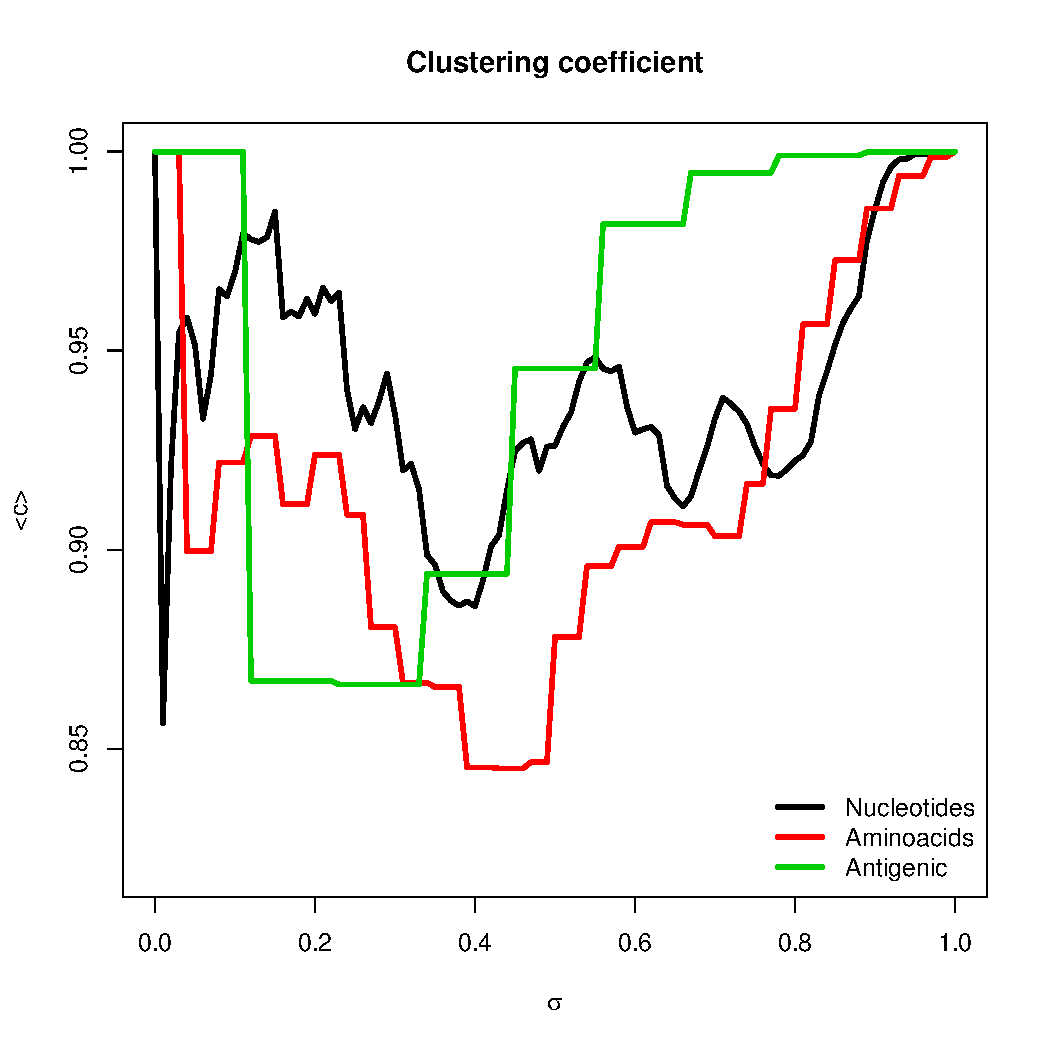
\includegraphics[scale=.35]{figures/clustering.pdf}}
\subfigure[$\langle k \rangle$]{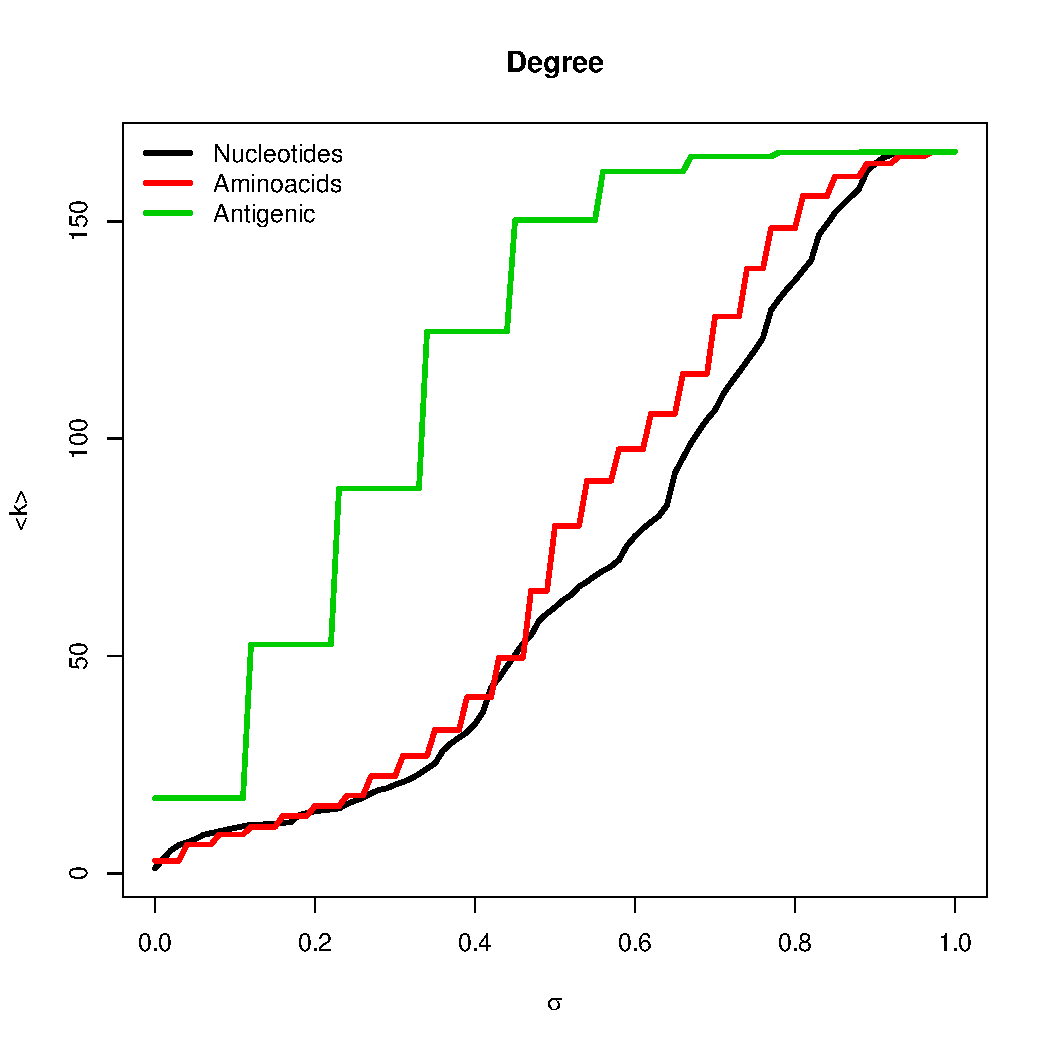
\includegraphics[scale=.35]{figures/degree.pdf}}\\
\subfigure[$L$]{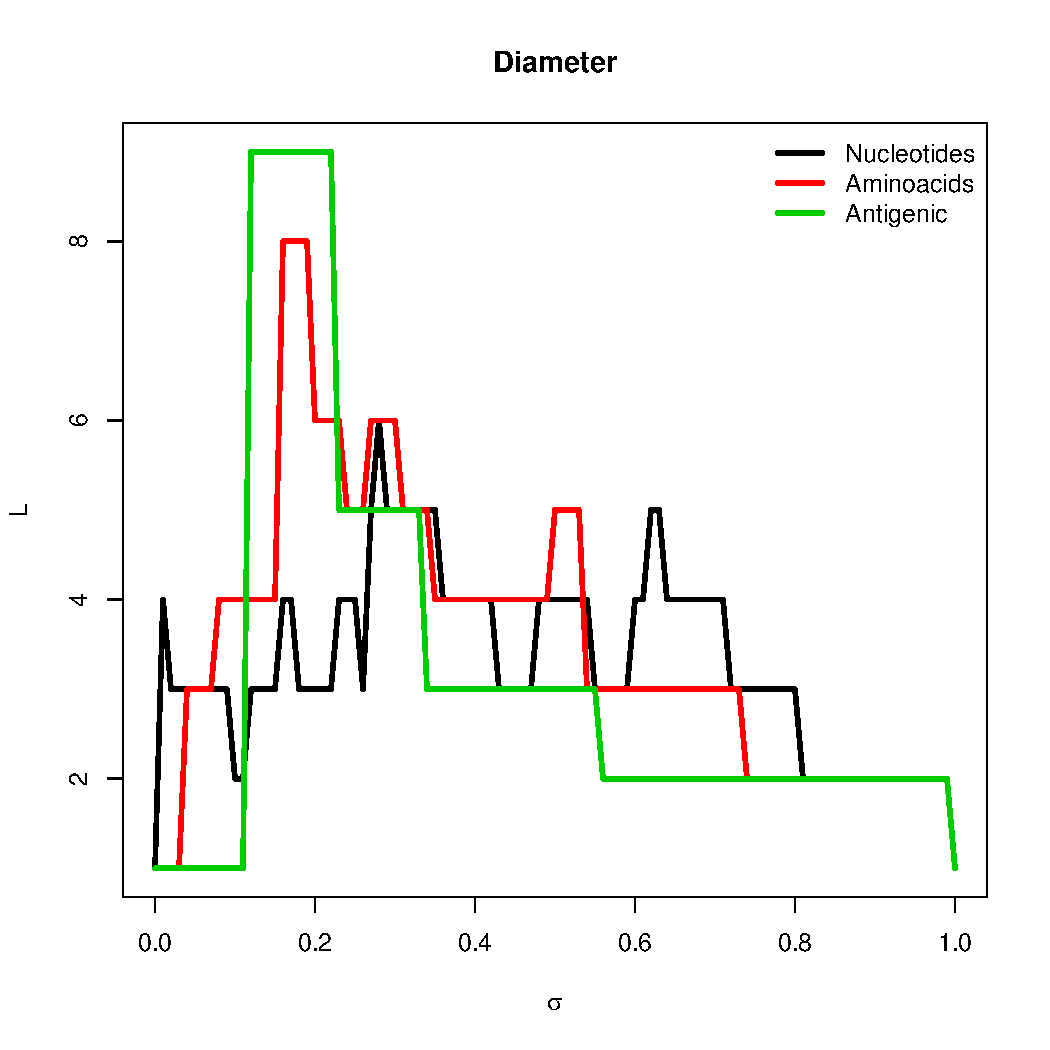
\includegraphics[scale=.35]{figures/diameter.pdf}}
\subfigure[$\langle l\rangle$]{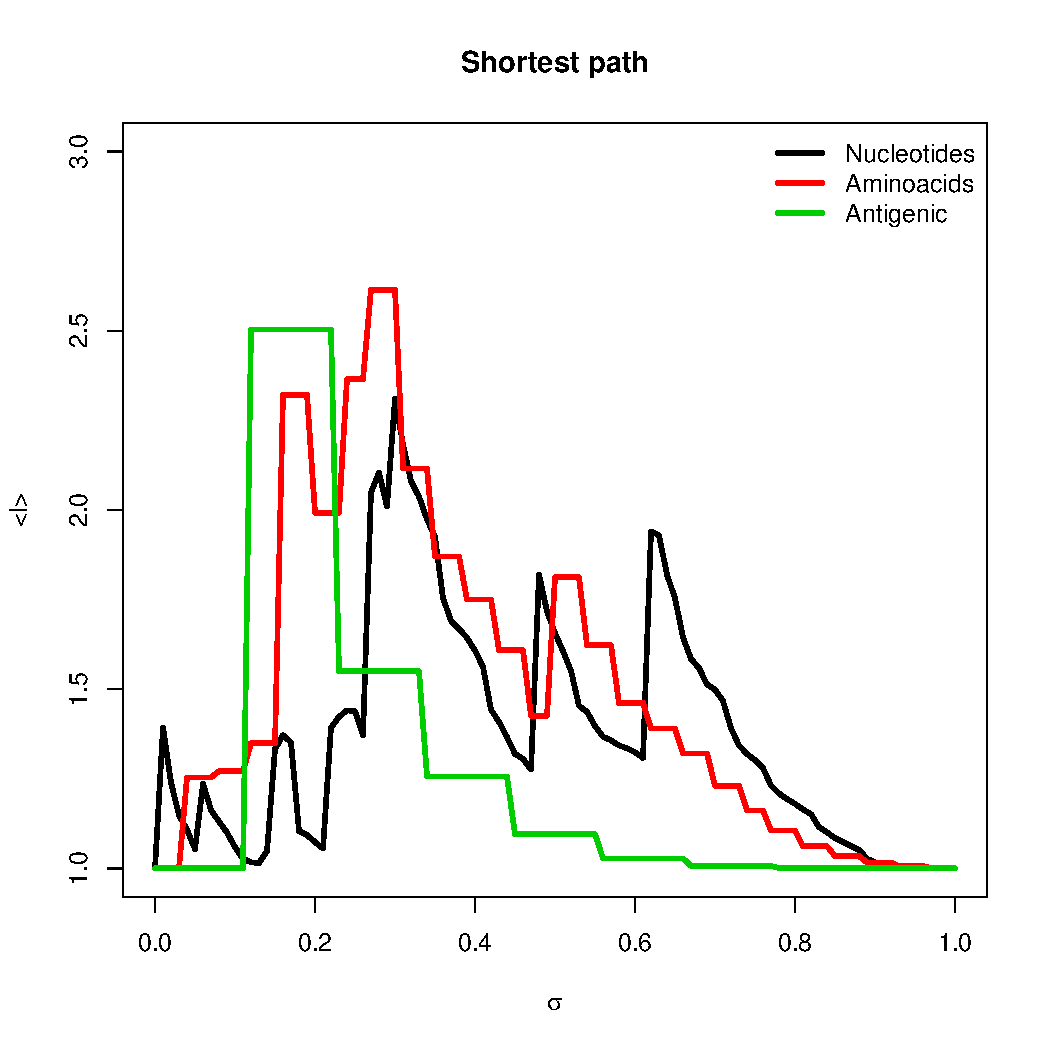
\includegraphics[scale=.35]{figures/spath.pdf}}\\
\subfigure[$r^{n}$]{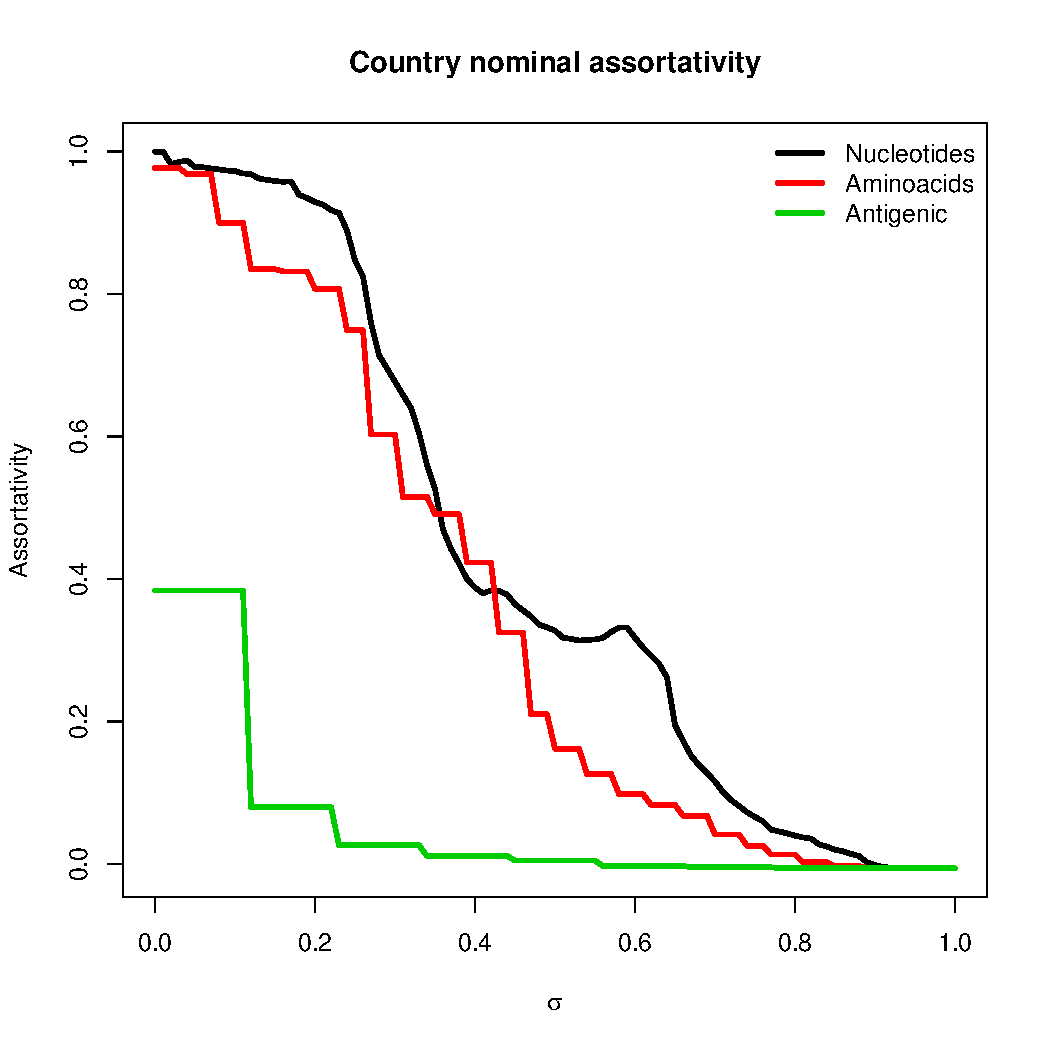
\includegraphics[scale=.35]{figures/country_assort.pdf}}
\subfigure[$r^{d}$]{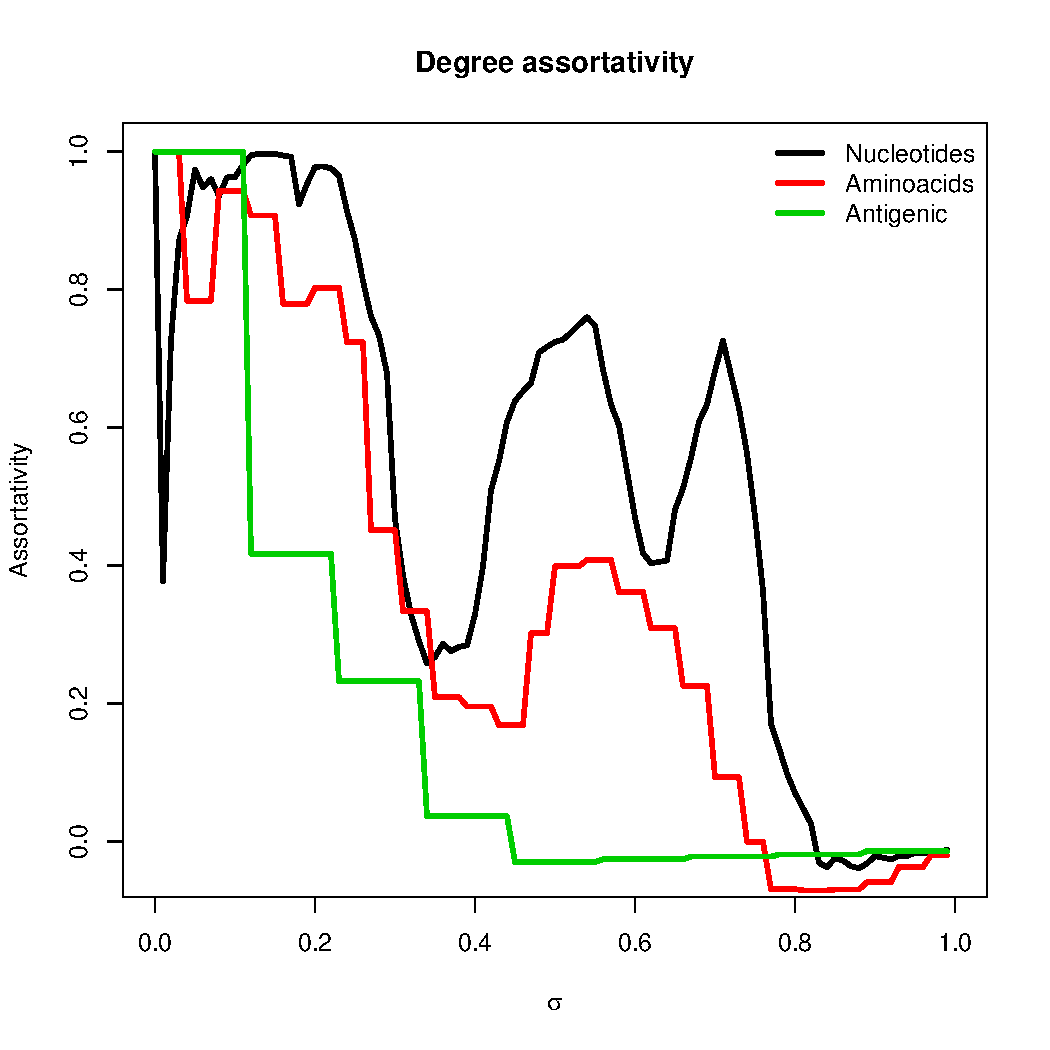
\includegraphics[scale=.35]{figures/degree_assort.pdf}}
\end{center}
\caption{\footnotesize Network indexes for the three data sets analyzed.
In panel (a) we show the clustering coefficient for each family of networks as a function of the threshold $\sigma$ and panel (b) shows the mean vertex degree.
Panels (c) and (d) show graph assortativity by vertex country and vertex degree, respectively.}
\label{fig:indexes}
\end{figure}
\end{center}
\newpage
%%%%%%%%%%%%%%%%%%%
Indexes for each $\sigma$ for the three data sets (NT, AA and ANT)  are presented in Figure~\ref{fig:indexes}
\begin{table}[!ht]
 \begin{center}
 \caption{\footnotesize Topological measures for the nucleotides (NT) data set.}
  \begin{tabular}{ccccc}
\toprule
  Network measure & \multicolumn{4}{c}{Threshold}\\
 & $\sigma=$& $\sigma=$& $\sigma=$&$\sigma=$\\
 \midrule
 $\langle k \rangle$ &     &          &          & \\
$\langle c \rangle$ &     &          &          & \\
$\langle l \rangle$ &     &          &          & \\ % shortest path
  $L$ &     &          &          & \\ % diameter
$r^{n}$ &   &          &          & \\ % assortativity country
$r^{d}$ &   &          &          & \\ % assortativity degree
\bottomrule
  \end{tabular}
 \end{center}
 \label{tab:indNT}
\end{table}
%%%%%%%%%%%%%%%%%
\begin{figure}[!ht]
\subfigure[$\sigma=$]{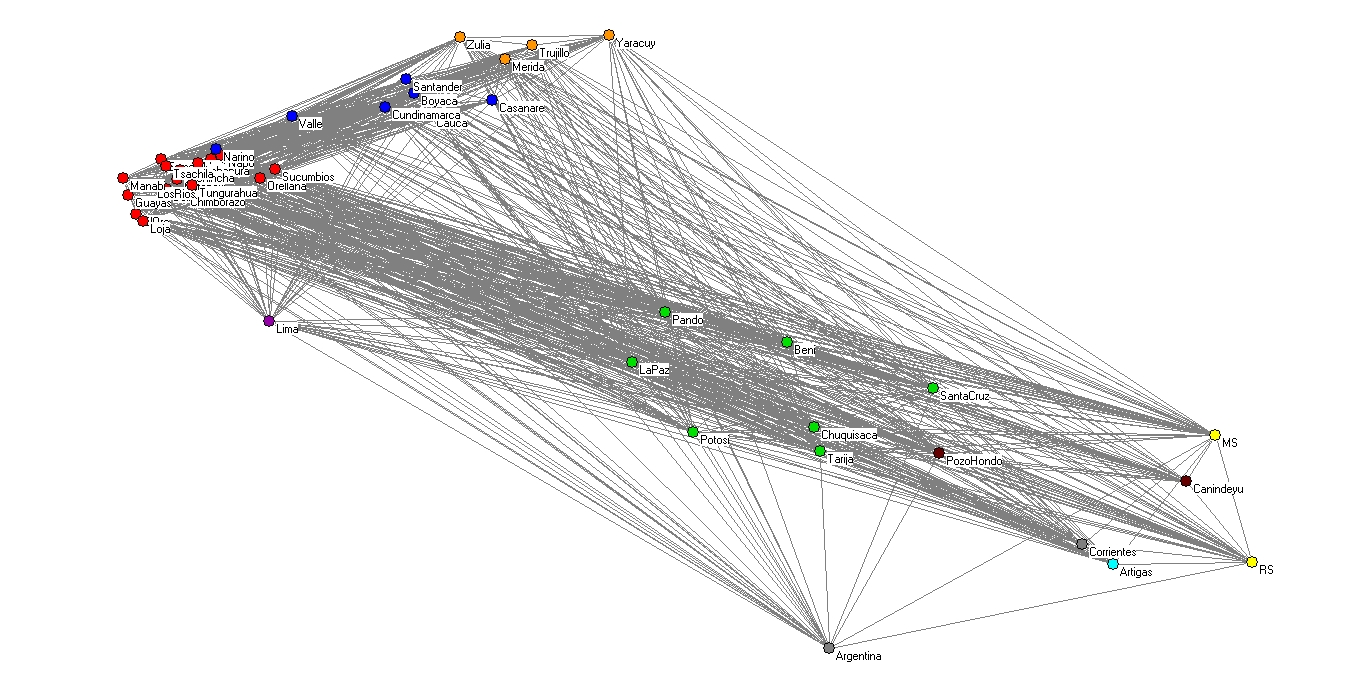
\includegraphics[scale=.15]{figures/net_NT_1.jpg}}
\subfigure[$\sigma=$]{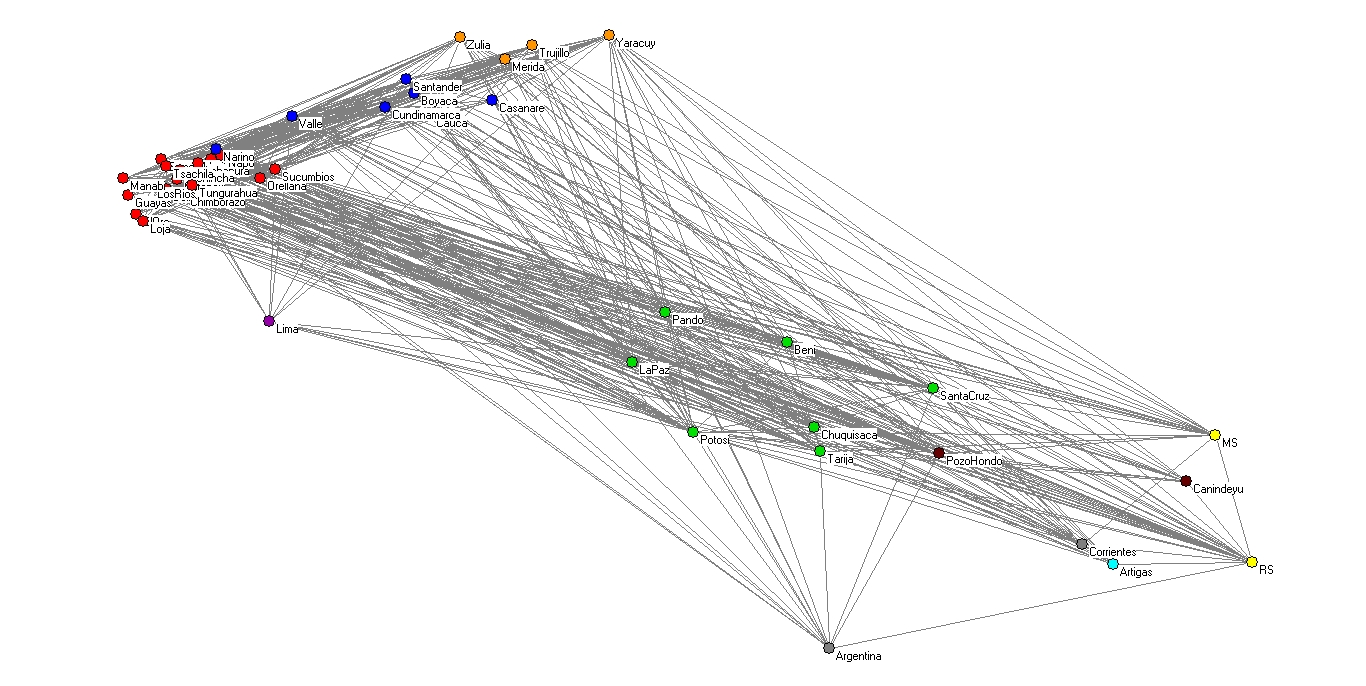
\includegraphics[scale=.15]{figures/net_NT_2.jpg}}\\
\subfigure[$\sigma=$]{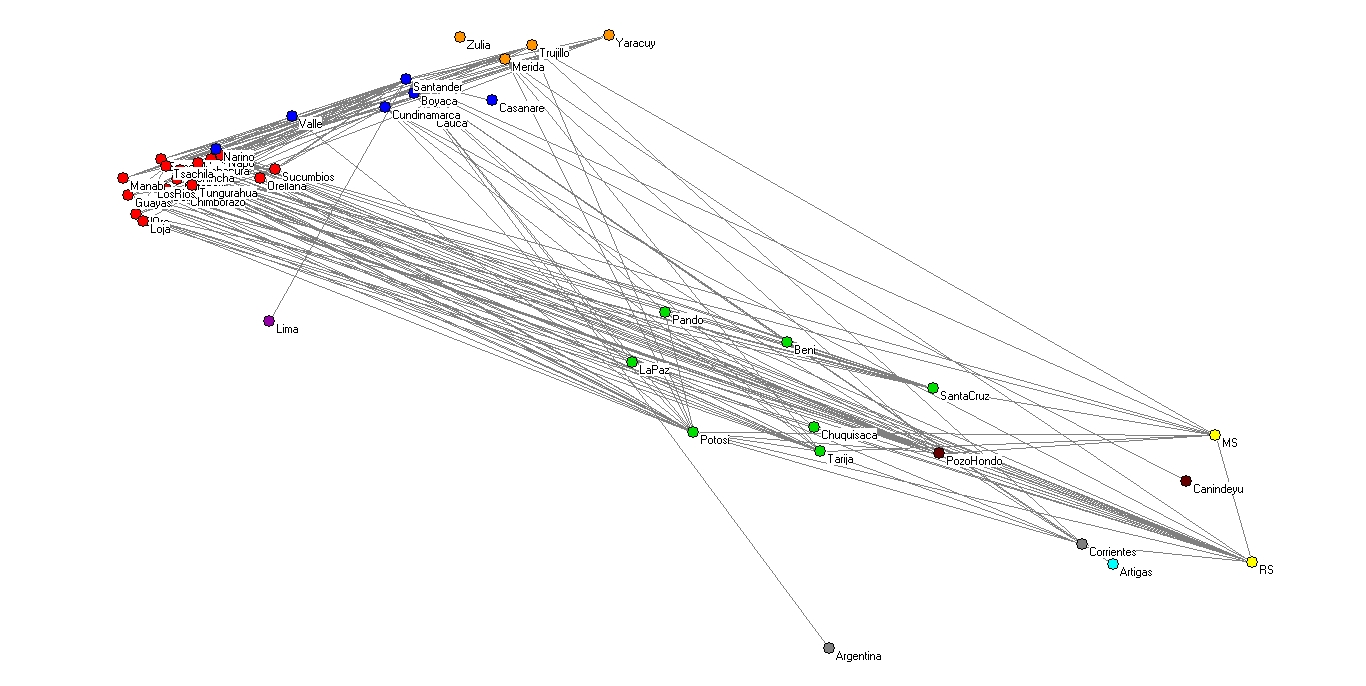
\includegraphics[scale=.15]{figures/net_NT_3.jpg}}
\subfigure[$\sigma=$]{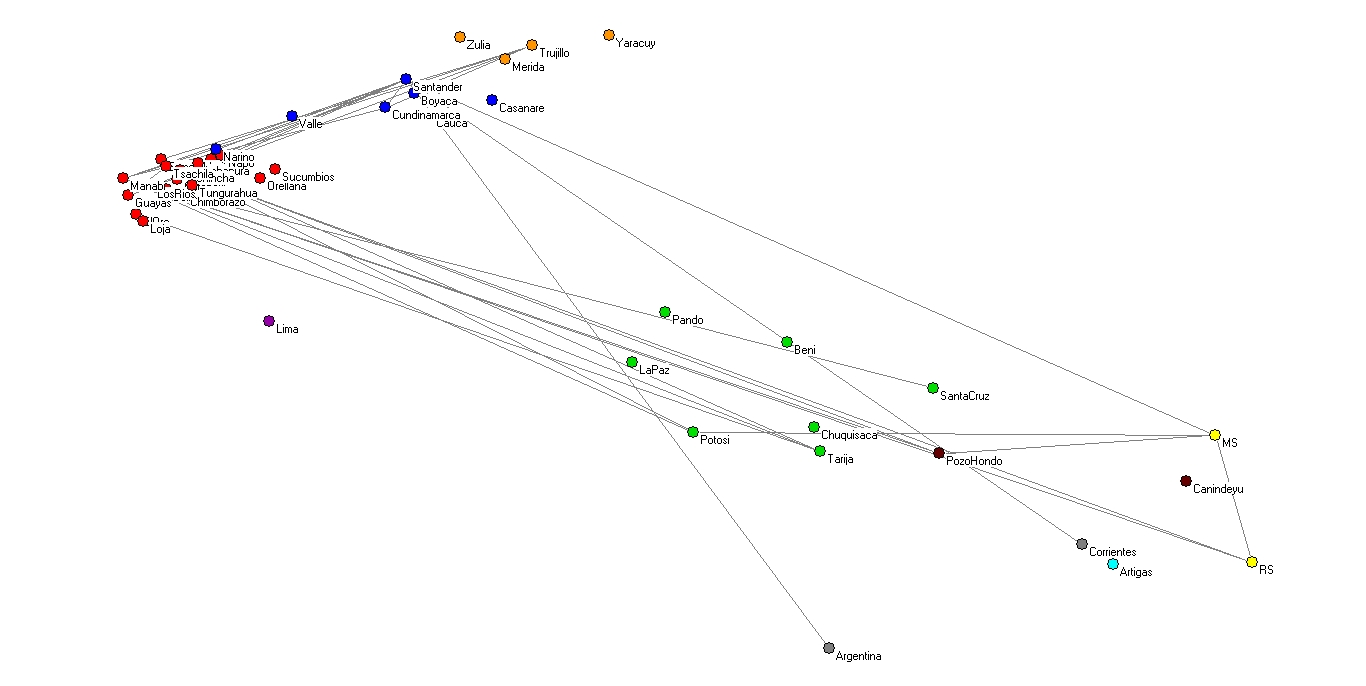
\includegraphics[scale=.15]{figures/net_NT_4.jpg}}
\caption{\footnotesize Georeferenced networks at critical values of $\sigma$ for the NT data set.
Vertices were colored according to}
\label{fig:netsNT}
\end{figure}
%%%%%%%%%%%%%%%%%
\begin{table}[!ht]
 \begin{center}
 \caption{\footnotesize Topological measures for the amino acids (AA) data set.}
  \begin{tabular}{ccccc}
\toprule
  Network measure & \multicolumn{4}{c}{Threshold}\\
 & $\sigma=$& $\sigma=$& $\sigma=$&$\sigma=$\\
 \midrule
$\langle k \rangle$ &     &          &          & \\
$\langle c \rangle$ &     &          &          & \\
$\langle l \rangle$ &     &          &          & \\ % shortest path
  $L$ &     &          &          & \\ % diameter
$r^{n}$ &   &          &          & \\ % assortativity country
$r^{d}$ &   &          &          & \\ % assortativity degree
\bottomrule
  \end{tabular}
 \end{center}
 \label{tab:indAA}
\end{table}
%%%%%%%%%%%%%%%%%
%%%%%%%%%%%%%%%%%
\begin{figure}[]
\subfigure[$\sigma=$]{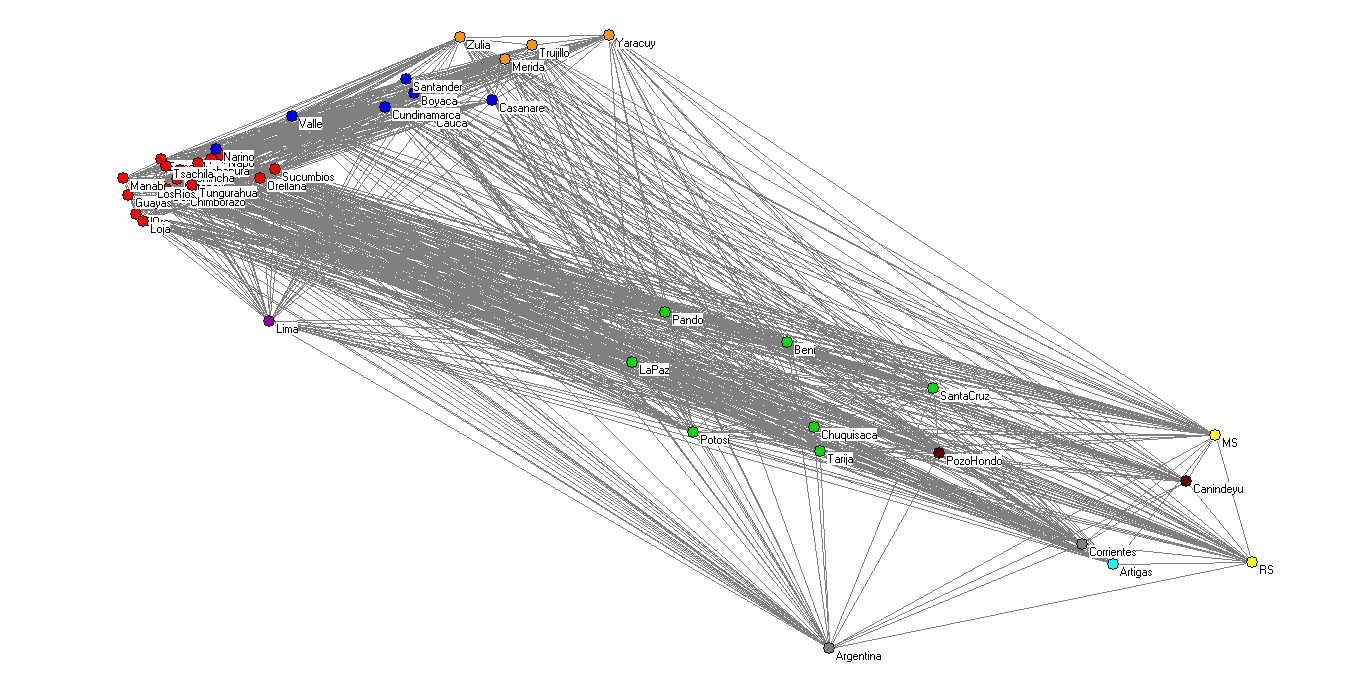
\includegraphics[scale=.15]{figures/net_AA_1.jpg}}
\subfigure[$\sigma=$]{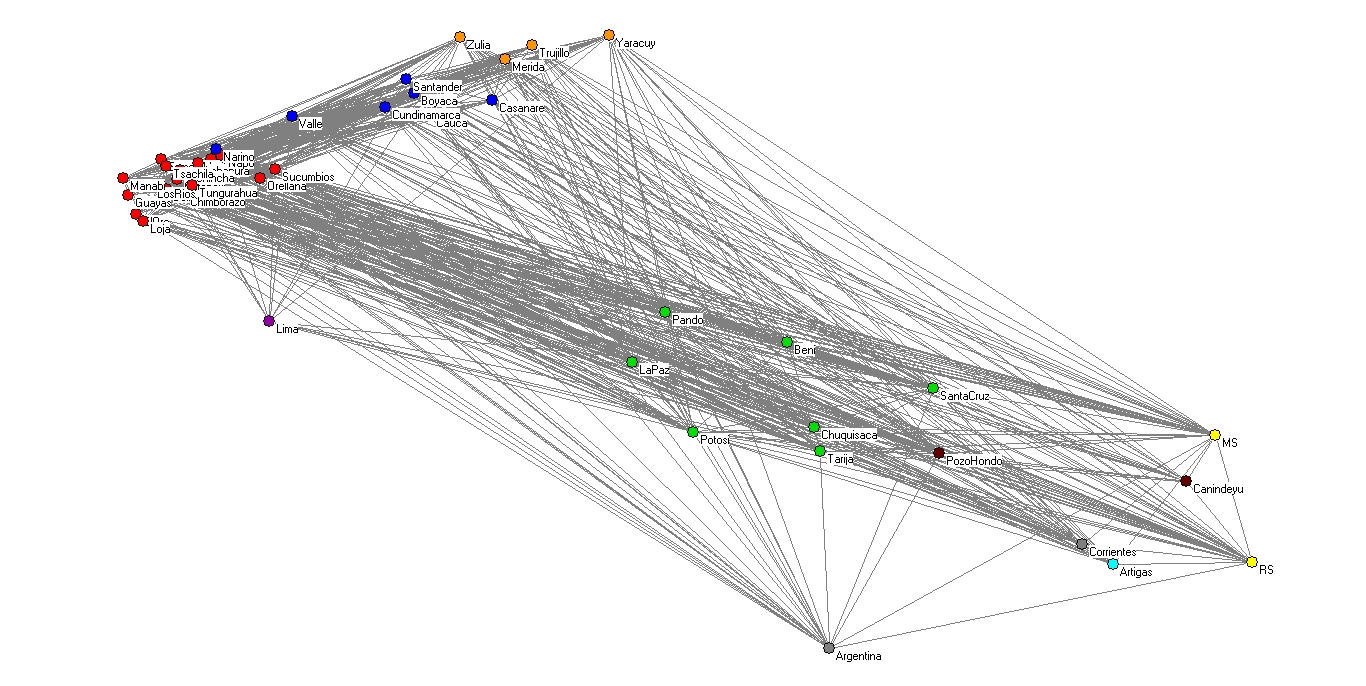
\includegraphics[scale=.15]{figures/net_AA_2.jpg}}\\
\subfigure[$\sigma=$]{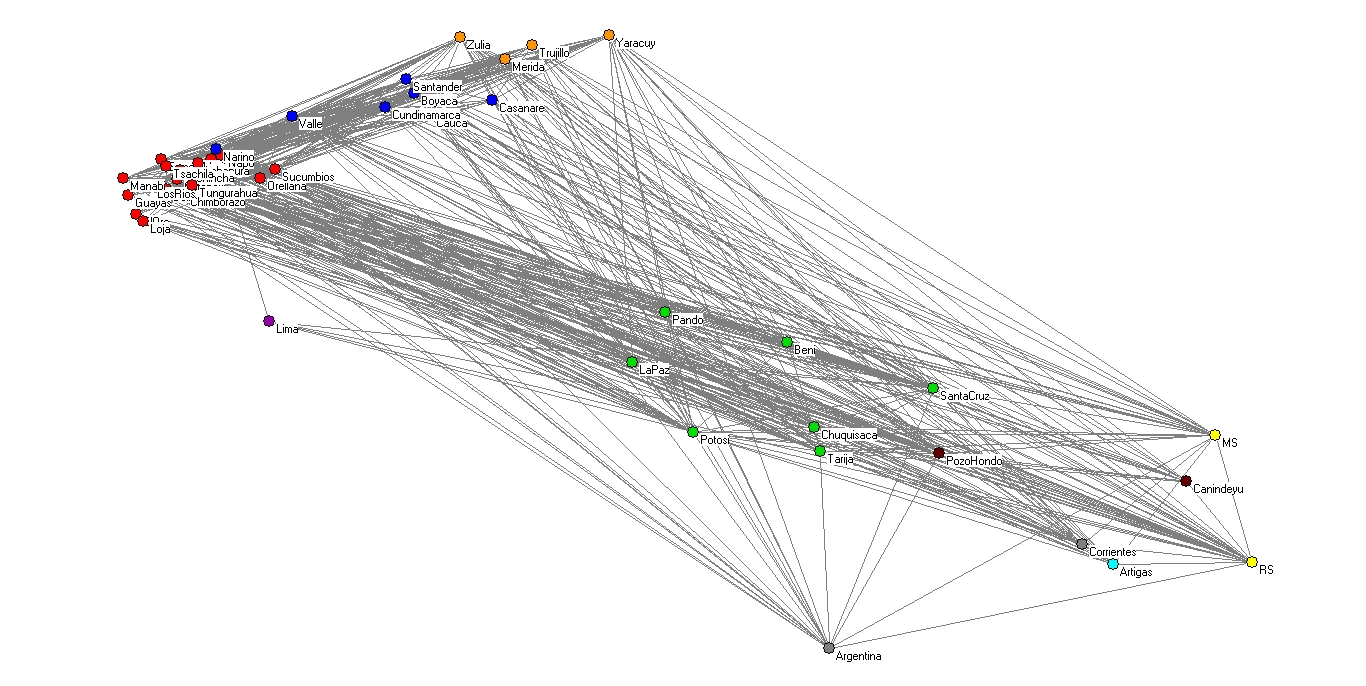
\includegraphics[scale=.15]{figures/net_AA_3.jpg}}
\subfigure[$\sigma=$]{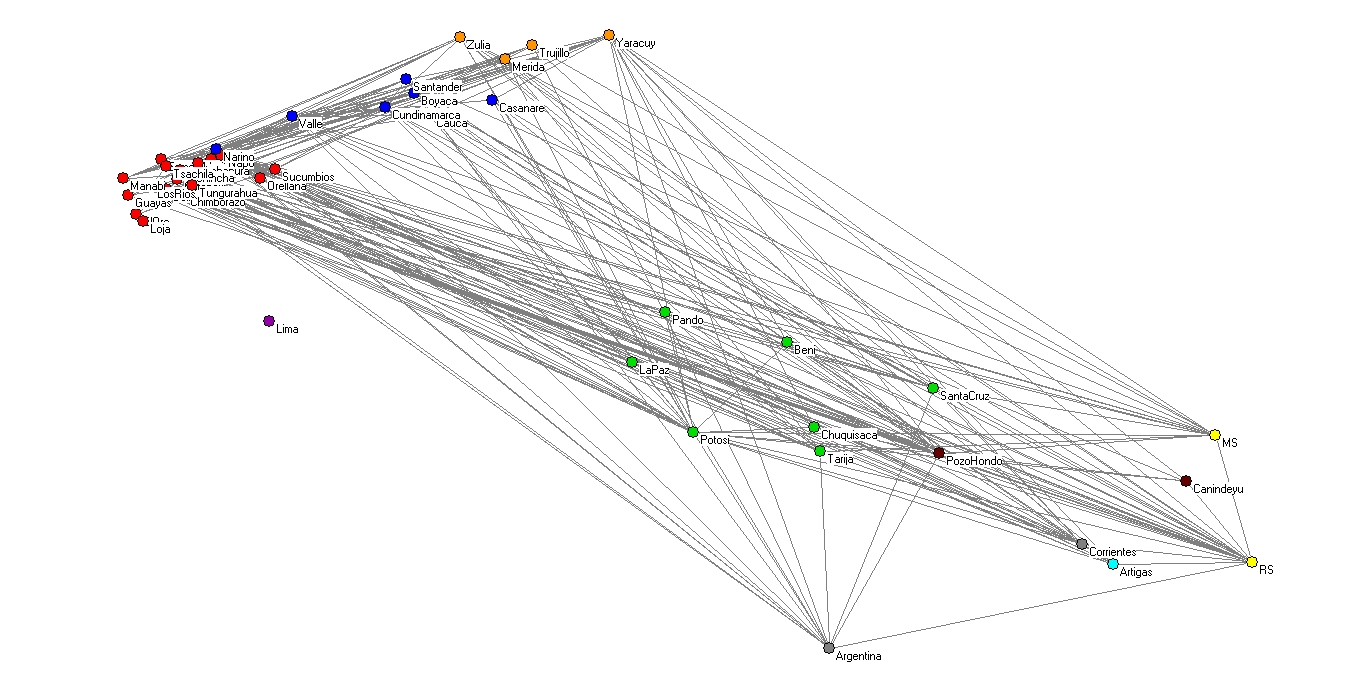
\includegraphics[scale=.15]{figures/net_AA_4.jpg}}
\caption{\footnotesize Georeferenced networks at critical values of $\sigma$ for the AA data set.
Vertices were colored according to}
\label{fig:netsAA}
\end{figure}
%%%%%%%%%%%%%%%%%
\begin{table}[]
 \begin{center}
 \caption{\footnotesize Topological measures for the VP1 antigenic region (ANT) data set.}
  \begin{tabular}{ccccc}
\toprule
  Network measure & \multicolumn{4}{c}{Threshold}\\
 & $\sigma=$& $\sigma=$& $\sigma=$&$\sigma=$\\
 \midrule
$\langle k \rangle$ &     &          &          & \\
$\langle c \rangle$ &     &          &          & \\
$\langle l \rangle$ &     &          &          & \\ % shortest path
  $D$ &     &          &          & \\ % diameter
$r^{n}$ &   &          &          & \\ % assortativity country
$r^{d}$ &   &          &          & \\ % assortativity degree
\bottomrule
  \end{tabular}
 \end{center}
 \label{tab:indANT}
\end{table}
%%%%%%%%%%%%%%%%%
%%%%%%%%%%%%%%%%%
\begin{figure}[t]
\subfigure[$\sigma=$]{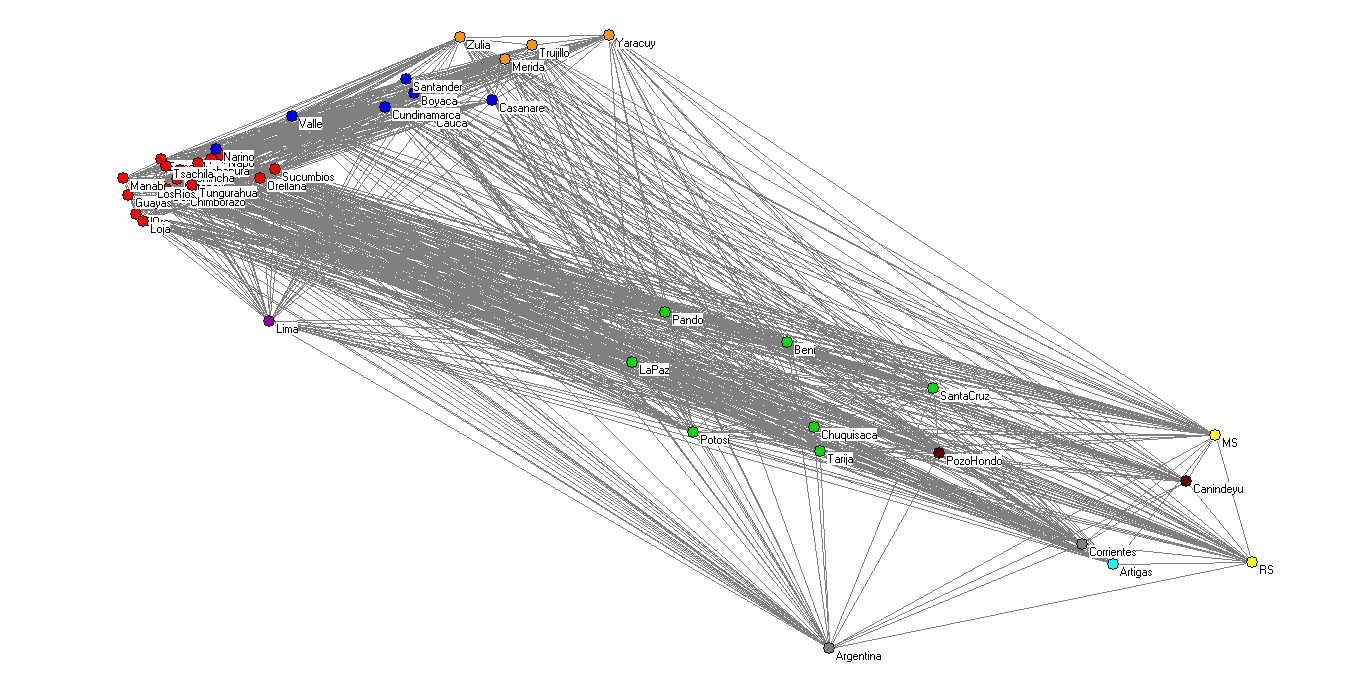
\includegraphics[scale=.15]{figures/net_ANT_1.jpg}}
\subfigure[$\sigma=$]{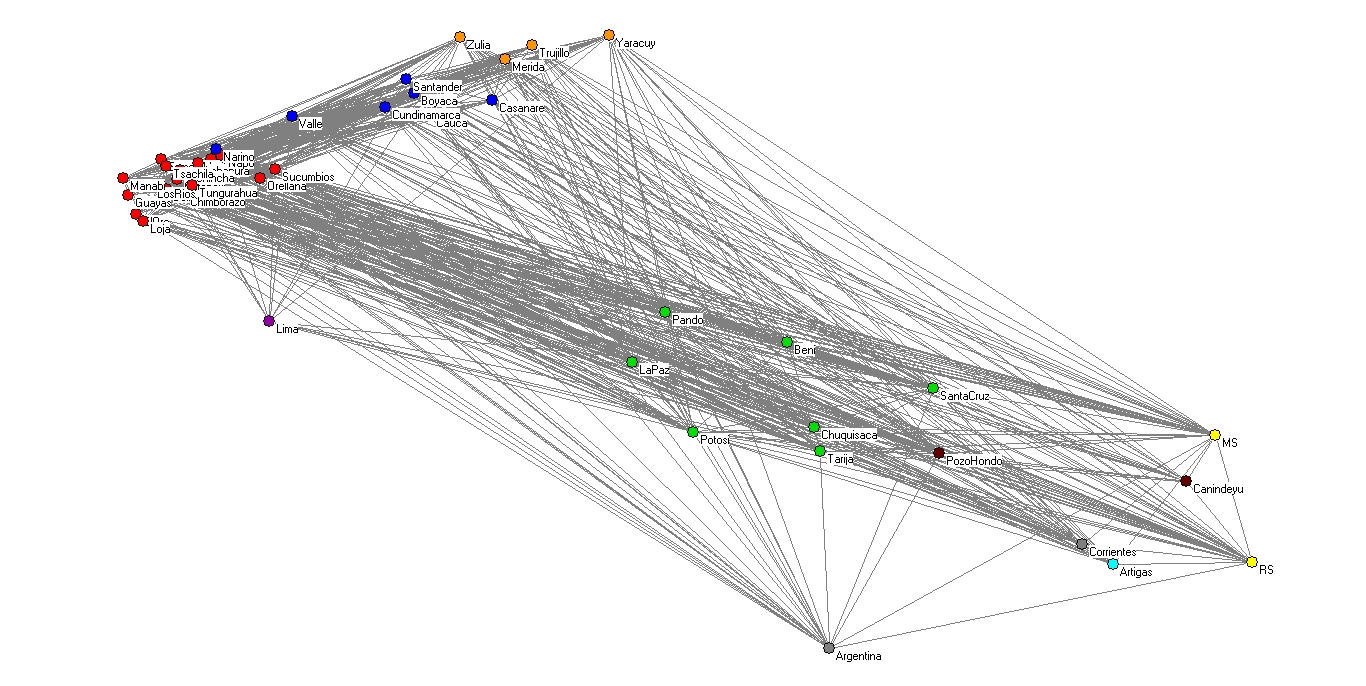
\includegraphics[scale=.15]{figures/net_ANT_2.jpg}}\\
\subfigure[$\sigma=$]{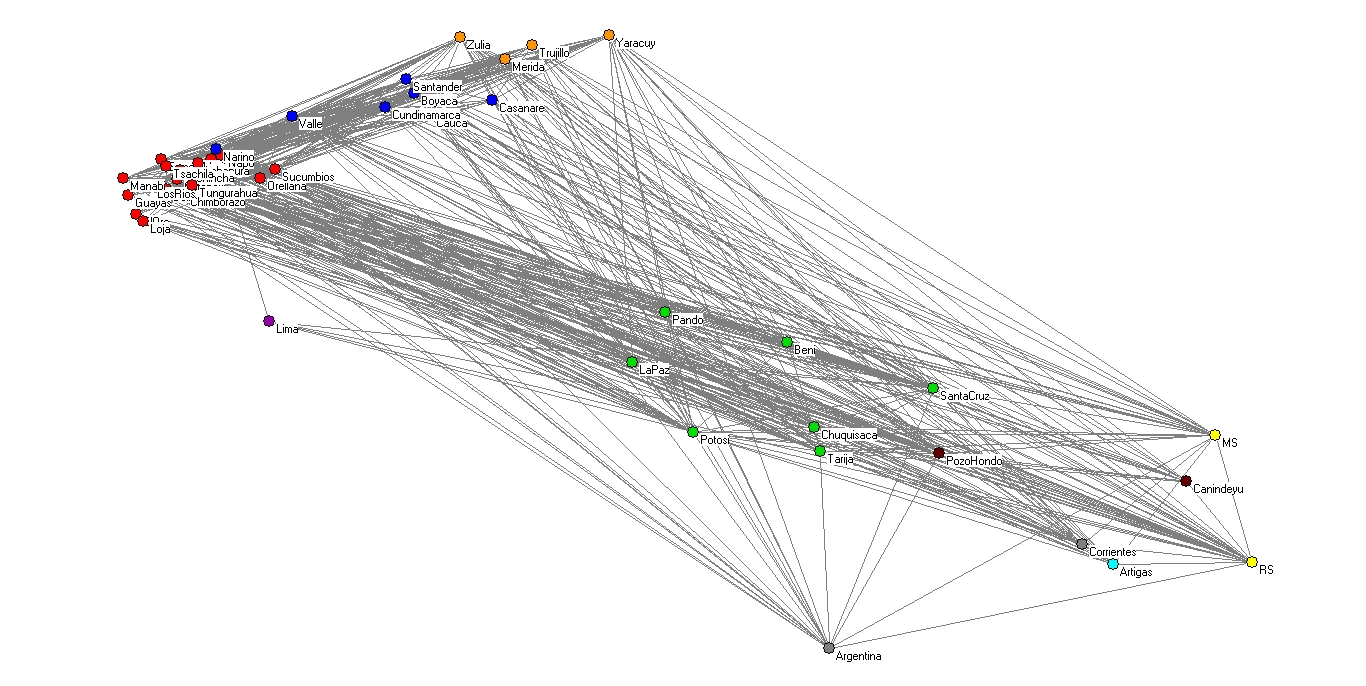
\includegraphics[scale=.15]{figures/net_ANT_3.jpg}}
\subfigure[$\sigma=$]{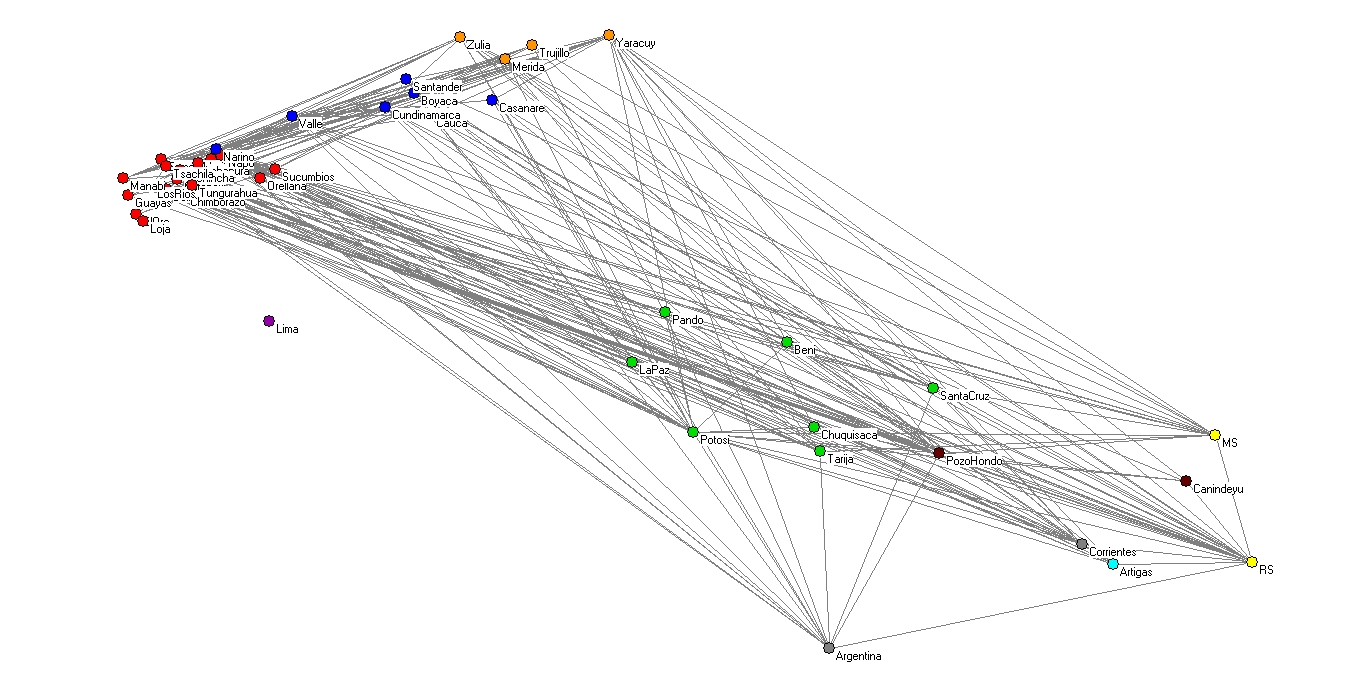
\includegraphics[scale=.15]{figures/net_ANT_4.jpg}}
\caption{\footnotesize Georeferenced networks at critical values of $\sigma$ for the antigenic region (ANT) data set.
Vertices were colored according to}
\label{fig:netsANT}
\end{figure}
%%%%%%%%%%%%%%%%%
\bigskip
\bigskip

\textbf{4. CONCLUSIONS AND PERSPECTIVES}

\bigskip
\bigskip
% computationally cheap \cite{Andrade2011}
We have demonstrated that complex networks can be used to explore viral genomic data and retrieve sound biological and epidemiological information.
% Further mathematical analysis is needed/ better theoretical study is due /...
\bigskip
\bigskip

{\bf ACKNOWLEDGMENTS: We thank Miguel Carvalho for operational support.}

\newpage
\bibliography{networks_FMDV}
\end{document}
